%**
%*  @file  agent_scheduler.tex
%*  @brief   DIET User's Manual: agent schedulers  
%*  @author  - Gael Le Mahec (gael.le.mahec@u-picardie.fr)
%*  @section Licence 
%*    |LICENSE|

\section{Scheduler at agents level}
In this section we introduce the way to define a scheduling policy in \diet.
Some scheduling strategies could not be developed using only the \diet {\sed}s
plugins. The schedulers at agents level allow the developer to design every
scheduler strategies, even the centralized ones. The first two sections
explain precisely how \diet performs the scheduling. The third section enters
in the \diet source code and can be ignored by most of the users. The
fourth section presents the tools provided to make an agent scheduler
easily. The fifth section deals with the scheduler module compilation and
usage. The last section presents some scheduler examples.
\subsection{Scheduling from the agents side.}
In \diet, the scheduling works as follows (see Figure \ref{scheduleSteps} for
a representation of each step): 
\begin{itemize}
  \item A request is submitted to the Master Agent (step 1).
  \item The Master Agent forwards the request to the Local Agents and {\sed}s that
    it manages (step 2).
  \item The {\sed}s which dispose of the asked service return a CORBA response
    structure which contains an estimation metric vector (step 3).
  \item According to a default policy or a user-defined one, the responses
    from the {\sed}s are aggregated. Then the responses sequence is sent to
    the parent agent which aggregates all the results of its children (step 4).
  \item When the aggregated responses reach the Master Agent, it returns
    the aggregated list of all responses to the client (step 5).
  \item Finally, the client chooses the better server, according to the
    chosen aggregation method (step 6).
\end{itemize}
\newlength{\schdlFigWidth}
\setlength{\schdlFigWidth}{(\textwidth - 3mm) / 3}
\begin{figure}[h]
  \centering
  \begin{minipage}{\schdlFigWidth}
    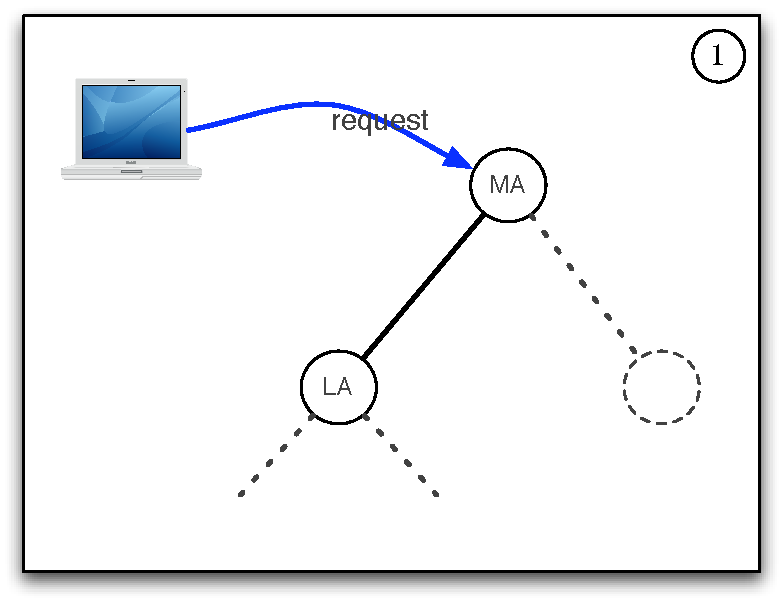
\includegraphics[width=\schdlFigWidth]{fig/schdl00}
  \end{minipage}
  \begin{minipage}{\schdlFigWidth}
    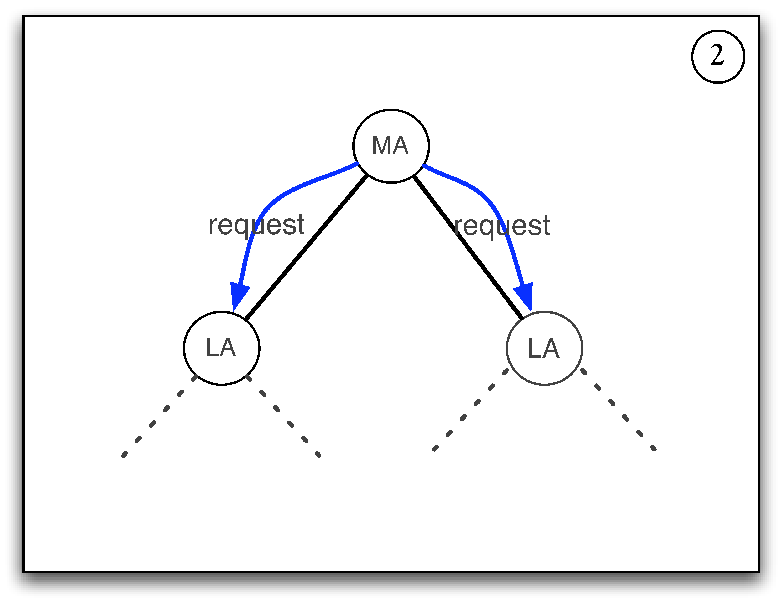
\includegraphics[width=\schdlFigWidth]{fig/schdl01}
  \end{minipage}
  \begin{minipage}{\schdlFigWidth}
    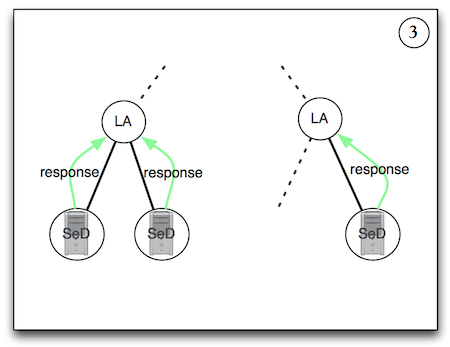
\includegraphics[width=\schdlFigWidth]{fig/schdl02}
  \end{minipage}\\
  \begin{minipage}{\schdlFigWidth}
    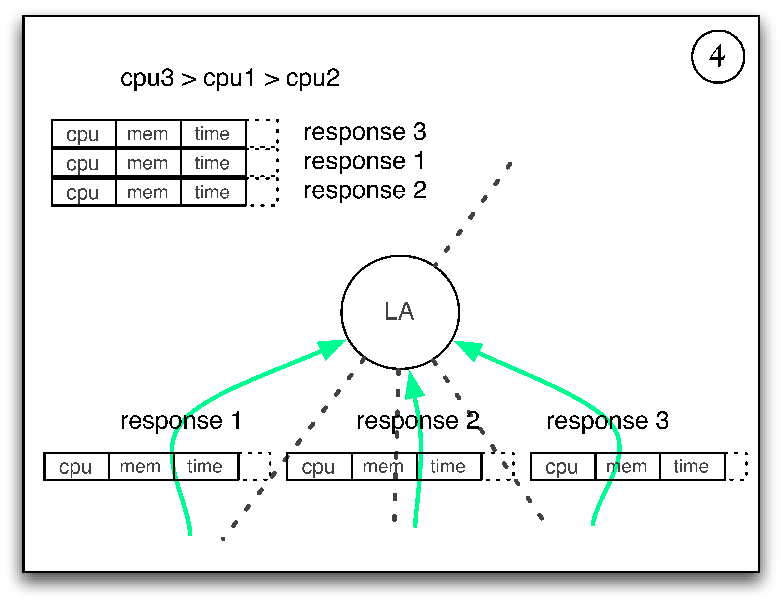
\includegraphics[width=\schdlFigWidth]{fig/schdl03}
  \end{minipage}
  \begin{minipage}{\schdlFigWidth}
    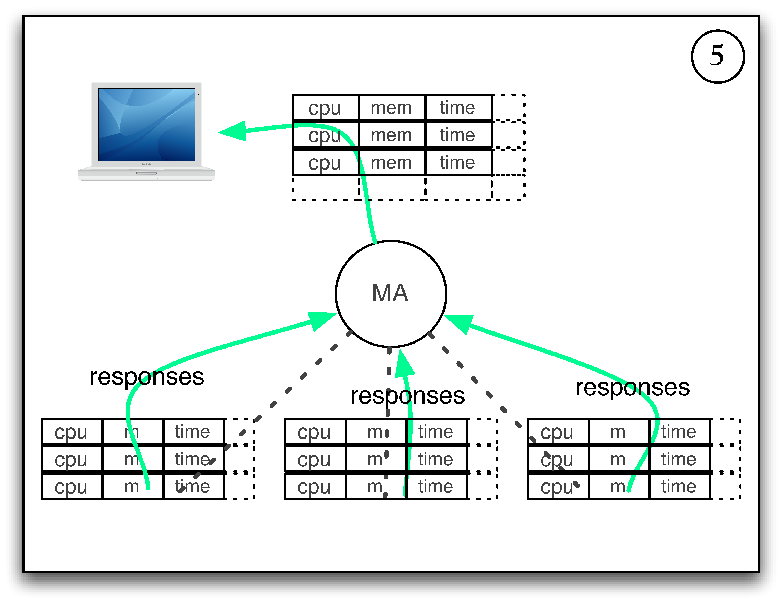
\includegraphics[width=\schdlFigWidth]{fig/schdl04}
  \end{minipage}
  \begin{minipage}{\schdlFigWidth}
    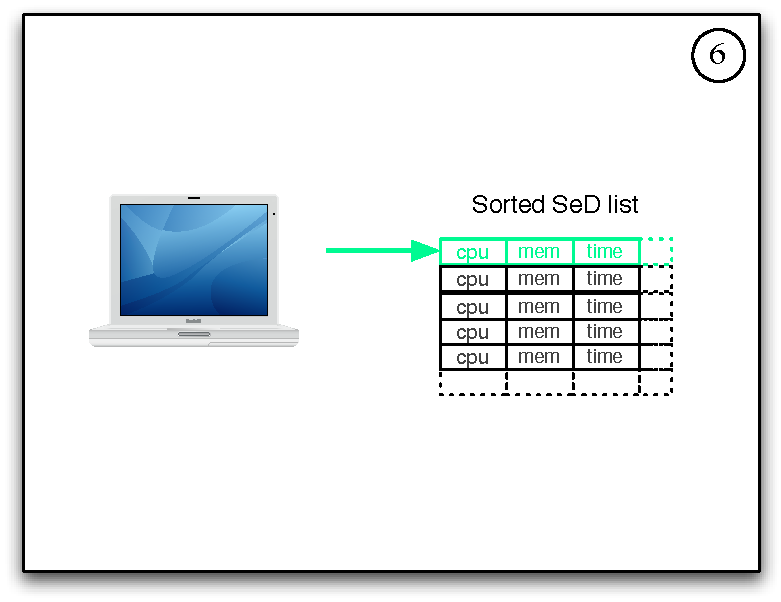
\includegraphics[width=\schdlFigWidth]{fig/schdl05}
  \end{minipage}
  \caption{Scheduling steps in \diet.\label{scheduleSteps}}
\end{figure}

\subsection{Aggregation methods overloading}
To aggregate the responses of the {\sed}s, \diet uses an aggregation method
which is called by the agents. This method is chosen from the {\sed}s
by defining the aggregator type (see Section \ref{sect:estTags}).
By default, two aggregator types are proposed by \diet:
DIET\_AGG\_DEFAULT and DIET\_AGG\_PRIORITY. Another aggregator type is
also available: DIET\_AGG\_USER. Using this
aggregator, the user can define her own aggregation method to be used by
the agents. 
Figure \ref{fig:DIETScheduling} presents the global schedulers classes
organization in \diet. By choosing the DIET\_AGG\_USER aggregator, the user
commands the GlobalScheduler class to load an external module containing
a UserScheduler class overloading the \textit{aggregate} method.
\begin{figure}[h]
  \centering
  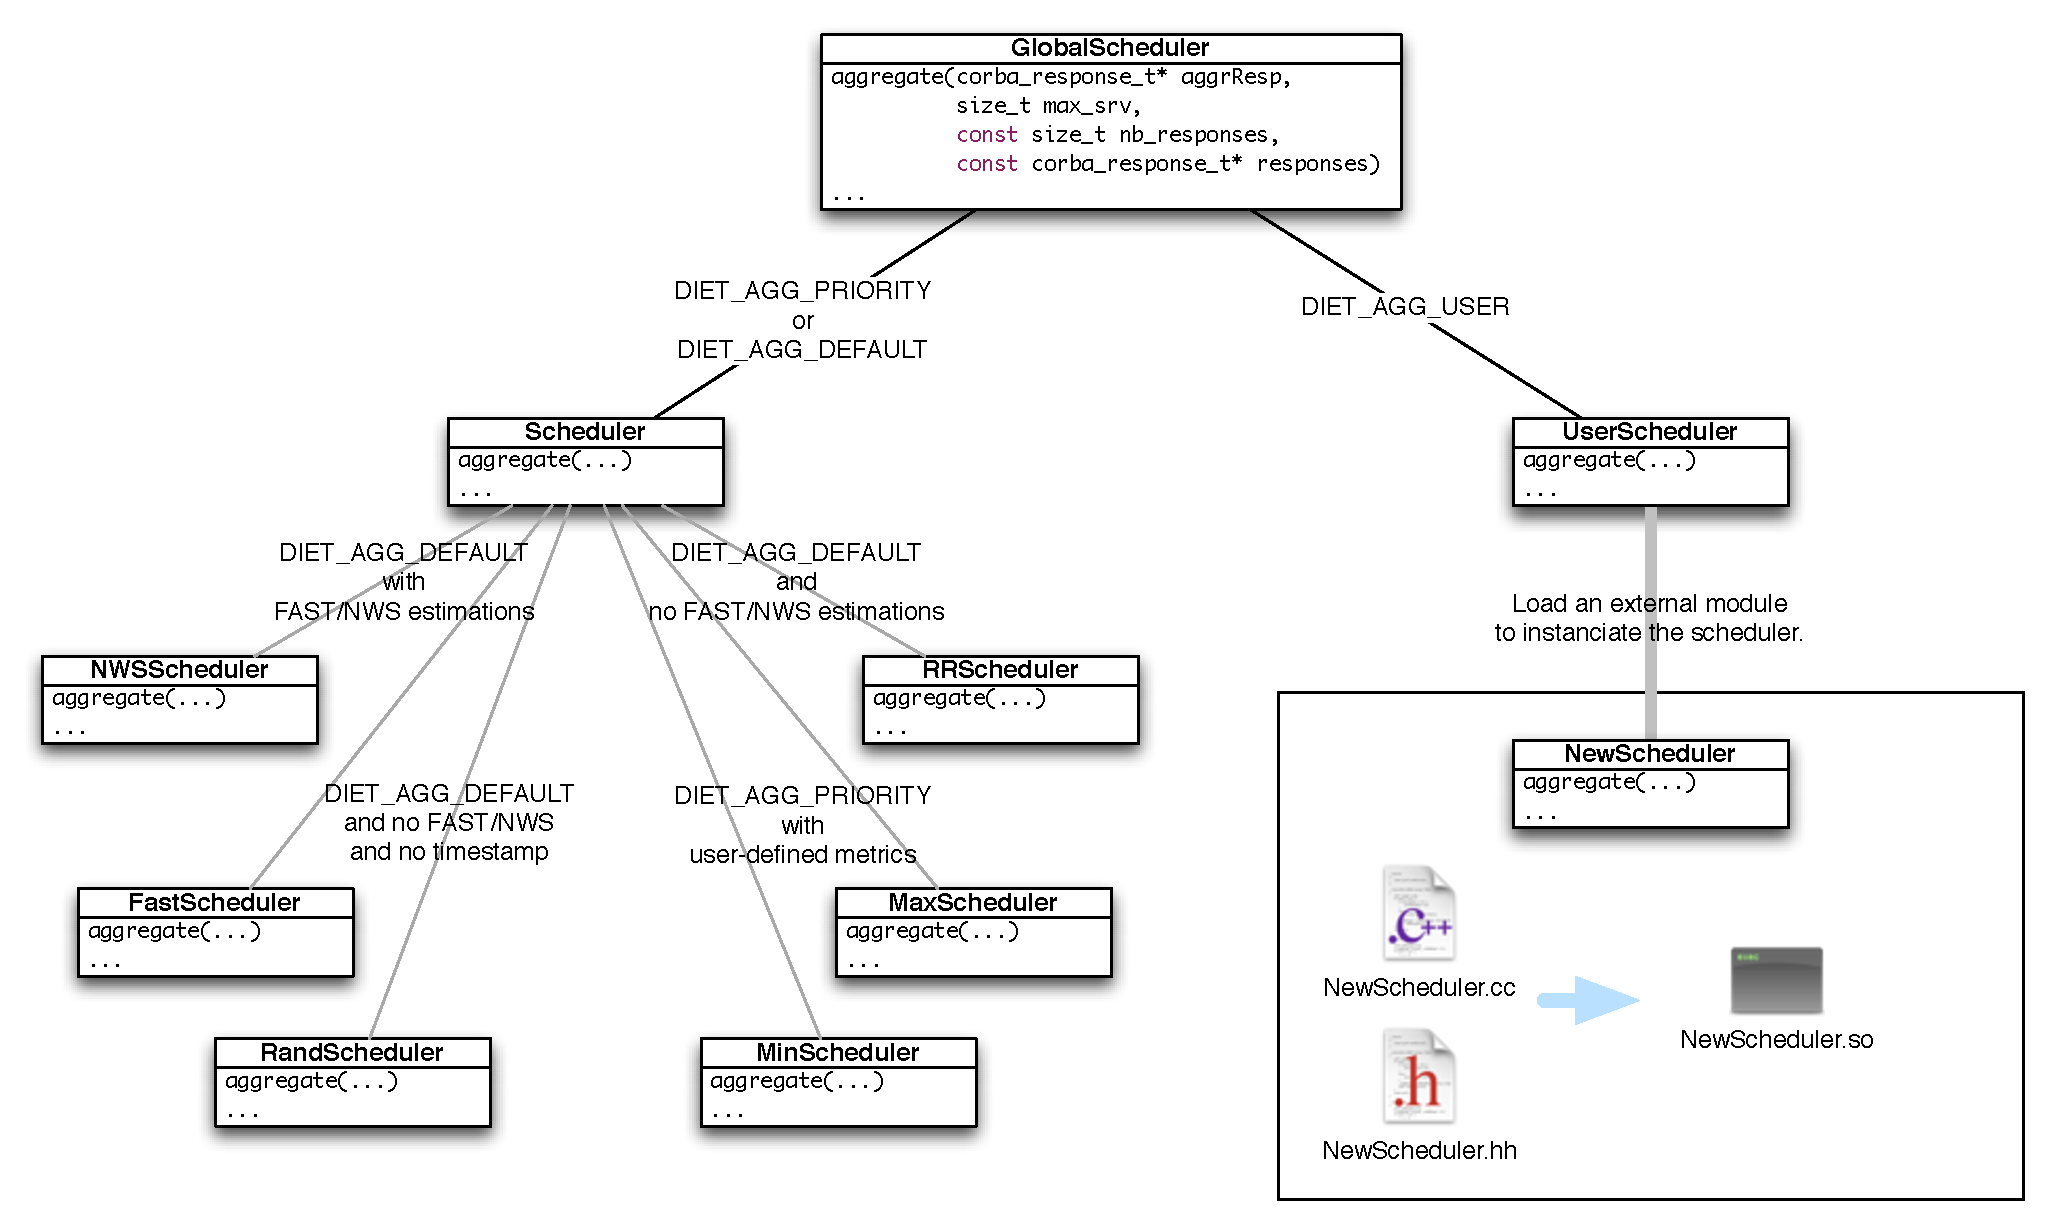
\includegraphics[width=16cm]{fig/DIETScheduling}
  \caption{Schedulers classes organization in \diet.\label{fig:DIETScheduling}}
\end{figure}

The user-defined aggregation method just needs to sort the responses from the
{\sed}s. By locating the aggregation method on the agent, we can use different
scheduling strategies which could not be implemented at the {\sed} level. These
schedulers can also avoid some scheduling problems while submitting asynchronous
jobs (with ``least recently used'' scheduler for example).

\subsection{The UserScheduler class}
This section presents how the scheduling process is managed in \diet.
Most of the developers can go directly to the next section.

All the schedulers developed by users have to inherit from the
\textit{UserScheduler} class. This class furnishes the methods to load
its subclasses as a Scheduler class for \diet without error. The only method
a user has to overload is the \textit{aggregate} method. Several useful
functions and macros are defined in the \textit{UserScheduler.hh} file.
The \textit{UserScheduler} class is defined as follows:
\begin{verbatim}
class UserScheduler : public GlobalScheduler
{
  typedef GlobalScheduler* constructor();
  typedef void destructor(UserScheduler*);

public:
  static const char* stName;
  UserScheduler();
  virtual
  ~UserScheduler();
  /** These methods are used to load the user module and to obtain an
     instance of the scheduler. */
  static UserScheduler* getInstance(const char* moduleName);
  static GlobalScheduler * instanciate(const char* moduleName);
  void destroy(GlobalScheduler* scheduler);

  static
  GlobalScheduler* deserialize(const char* serializedScheduler,
			       const char* moduleName);
  static
  char* serialize(GlobalScheduler* GS);
  /** The method that has to be overloaded to define a new scheduler. */
  virtual int
  aggregate(corba_response_t* aggrResp,
            size_t max_srv,
            const size_t nb_responses,
            const corba_response_t* responses);

private:
  /** The UserScheduler class is a singleton class. Its constructor is
   private. */
  UserScheduler(const char* moduleName);
  static UserScheduler* instance;
  void* module;
  /** These two methods are obtained from the loaded module. */
  constructor* constructs;
  destructor* destroys;
};
\end{verbatim}

\noindent The \textit{aggregate} method takes 4 arguments:
\begin{itemize}
  \item \textit{corba\_response\_t* \bf aggrResp}: the result of the aggregation
    has to be set in this argument. \textit{\bf aggrResp} is an array of
    \textit{corba\_server\_estimation\_t} objects. 
  \item \textit{size\_t \bf max\_srv}: this argument gives the maximum number
    of responses to return in \textit{\bf aggrResp}. This value can be ignored
    without any risk and it is sometimes useful to ignore it because this
    parameter is hard-coded in the \diet sources.
  \item \textit{const size\_t \bf nb\_responses}: this argument gives the number
    of responses in \textit{\bf responses}.
  \item \textit{const corba\_response\_t* \bf responses}: the responses are
    stored in this argument. It is an array of \textit{corba\_response\_t}
    which is a CORBA structure containing a CORBA sequence of
    \textit{corba\_server\_estimation\_t}.
\end{itemize}

\noindent The \textit{corba\_response\_t} structure is defined as follows:
\begin{verbatim}
struct corba_response_t {
  typedef _CORBA_ConstrType_Variable_Var<corba_response_t> _var_type;  
  CORBA::ULong reqID;
  CORBA::Long myID;
  SeqServerEstimation_t servers;
  void operator>>= (cdrStream &) const;
  void operator<<= (cdrStream &);
};
\end{verbatim}

\noindent The \textit{\bf \_var\_type} field is an internal CORBA object. The
scheduler developer does not have to use it. The two operators
\textit{\bf operator$>>=$} and \textit{\bf operator$>>=$} can be ignored too.
\begin{itemize}
  \item \textit{CORBA::ULong \bf reqID}: this field contains the ID of the
    request.
  \item \textit{CORBA::Long \bf myID}: this field is for \diet internal usage.
    The developer should ignore it.
  \item \textit{SeqServerEstimation\_t \bf servers}: this field is a sequence
    of \textit{corba\_server\_estimation\_t}. It is used to store the {\sed}s
    references returned by the \textit{aggregate} method. This is the field
    that has to be sorted/filtered.
\end{itemize}

\noindent The \textit{corba\_server\_estimation\_t} is defined as follows:
\begin{verbatim}
struct corba_server_estimation_t {
  typedef _CORBA_ConstrType_Variable_Var<corba_server_estimation_t> _var_type;
  corba_server_t loc;
  corba_estimation_t estim;
  void operator>>= (cdrStream &) const;
  void operator<<= (cdrStream &);
};
\end{verbatim}
\begin{itemize}
  \item \textit{corba\_server\_t \bf loc}: this field is used to designate a
    particular {\sed}.
  \item \textit{corba\_estimation\_t estim}: this field contains the estimation
    vector for the designated {\sed}.
\end{itemize}

\noindent The \textit{corba\_server\_t \bf loc} structure is defined as
follows:
\begin{verbatim}
struct corba_server_t {
  typedef _CORBA_ConstrType_Variable_Var<corba_server_t> _var_type;  
  _CORBA_ObjRef_Member< _objref_SeD, SeD_Helper>  ior;
  CORBA::String_member hostName;
  CORBA::Long port;
  void operator>>= (cdrStream &) const;
  void operator<<= (cdrStream &);
};
\end{verbatim}
The two interesting fields are:
\begin{itemize}
  \item \textit{\bf ior} which is a CORBA reference to the {\sed}.
  \item \textit{\bf hostName} which is the hostname of the {\sed}.
\end{itemize}

\noindent The \textit{corba\_estimation\_t} structure is defined as follows:
\begin{verbatim}
struct corba_estimation_t {
  typedef _CORBA_ConstrType_Variable_Var<corba_estimation_t> _var_type;
  SeqEstValue_t estValues;
  void operator>>= (cdrStream &) const;
  void operator<<= (cdrStream &);
};
\end{verbatim}
\textit{SeqEstValue\_t \bf estValues}: This field is a CORBA sequence of
estimation values. These estimation values are accessed through the specific
functions: \textit{diet\_est\_get\_internal} and \linebreak
\textit{diet\_est\_array\_get\_internal} defined in scheduler/est\_internal.hh.

\noindent These functions prototypes are:
\begin{verbatim}
double diet_est_get_internal(estVectorConst_t ev, int tag, double errVal);
double diet_est_array_get_internal(estVectorConst_t ev, int tag,
                                   int idx, double errVal);
\end{verbatim}
\begin{itemize}
  \item \textit{ev}: the estimation vector to evaluate.
  \item \textit{tag}: the estimation tag.
  \item \textit{idx}: the index of the value when available. For example, to
    obtain the frequency of the second processor, we have to set $idx$ to 1.
  \item \textit{errVal}: the value returned by the function if an error
    occurred.
\end{itemize}

\noindent The \textit{tag} argument may be assigned one of the following values:
\begin{itemize}
  \item[-] EST\_TIMESINCELASTSOLVE: The time elapsed since this {\sed} solved
    a request. This value is used by the default Round-Robin scheduler when
    available.
  \item[-] EST\_COMMPROXIMITY:
  \item[-] EST\_TRANSFEREFFORT:
  \item[-] EST\_FREECPU: The free CPU computation power.
  \item[-] EST\_FREEMEM: The free memory on the node.
  \item[-] EST\_NBCPU: The number of CPU installed on the node.
  \item[-] EST\_CPUSPEED\footnote{This value is accessed using the
      \textit{diet\_est\_array\_get\_internal} function}: The frequencies
    of the CPUs of the node.
  \item[-] EST\_TOTALMEM: The total memory of the node.
  \item[-] EST\_AVGFREEMEM: The average free memory on the node.
  \item[-] EST\_AVGFREECPU: The average free CPU computation power on the node.
  \item[-] EST\_BOGOMIPS\footnotemark[\value{footnote}]: The computation power
    of the nodes CPUs given in bogomips.
  \item[-] EST\_TOTALSIZEDISK: The total disk size on the node.
  \item[-] EST\_FREESIZEDISK: The available disk space on the node.
  \item[-] EST\_DISKACCESREAD: An evaluation of the disk read access performance.
  \item[-] EST\_DISKACCESWRITE: An evaluation of the disk write access performance.
  \item[-] EST\_USERDEFINED: The first user-defined value.
  \item[-] EST\_USERDEFINED $+$ n: The n$^{th}$ user-defined value.
\end{itemize}

To make the new scheduler class loadable by the GlobalScheduler class, the
developer has to define these two functions outside the class definition:
\begin{verbatim}
extern "C" GlobalScheduler* constructor() {
    return new MyScheduler();
}
extern "C" void destructor(UserScheduler* scheduler) {
  delete scheduler;
}
\end{verbatim}
No C++ implementation of dynamic class loading are defined in the C++ standard.
So, the UserScheduler class has to use C functions to load an external module
containing the new scheduler class. A macro defined in \textit{UserScheduler.hh}
automates this declaration. You can simply define your class as a scheduler
class by calling \textit{SCHEDULER\_CLASS(MyScheduler)}, where
\textit{MyScheduler} is the name of the class which inherits of
the \textit{UserScheduler} class.

\subsection{Easy definition of a new scheduler class}
The previous section presented how the scheduler class loader is working. Many
things presented before can be automated. The UserScheduler.hh file defines
some useful functions and macros to make a new scheduler class easily. In this
section we will present how to create a new scheduler class using these
functions and macros.

\subsubsection{The new class definition}
Every scheduler class has to inherit from the UserScheduler class. The only
redefinition needed is the \textit{aggregate} function. But, the \textit{init},
\textit{serialize} and \textit{deserialize} functions have to be declared
conforming to the C++ standard (but not defined - the inherited functions are
sufficient). The following example shows a simple scheduler class
implementation.
\begin{verbatim}
class MyScheduler : public UserScheduler {
public:
  static const char* stName;

  MyScheduler();
  ~MyScheduler();
  void init();

  static char* serialize(MyScheduler* GS);
  static MyScheduler* deserialize(const char* serializedScheduler);
  /* Overriden UserScheduler class aggregate method. */
  int aggregate(corba_response_t* aggrResp, size_t max_srv,
                const size_t nb_responses, const corba_response_t* responses);
};

const char* MyScheduler::stName="UserGS";

MyScheduler::~MyScheduler() {

}

MyScheduler::MyScheduler() {
  this->name = this->stName;
  this->nameLength = strlen(this->name);
}

int MyScheduler::aggregate(corba_response_t* aggrResp, size_t max_srv,
                            const size_t nb_responses,
                            const corba_response_t* responses)
{
  ...
}

SCHEDULER\_CLASS(MyScheduler)
\end{verbatim}
After defining the scheduler class, the developer just has to use the
\textit{SCHEDULER\_CLASS} macro to define it as a scheduler class loadable
from an agent.

In our example, the call to \textit{SCHEDULER\_CLASS(MyScheduler)} --
after the class declaration -- makes the class loadable by a \diet agent.

\subsubsection{The aggregation method redefinition}
The \textit{aggregate} function has the following prototype:
\begin{verbatim}
int MyScheduler::aggregate(corba_response_t* aggrResp, size_t max_srv,
                            const size_t nb_responses,
                            const corba_response_t* responses)
{
  ...
}
\end{verbatim}

\noindent The \textit{aggregate} method takes 4 arguments:
\begin{itemize}
  \item \textit{corba\_response\_t* \bf aggrResp}: the result of the aggregation
    has to be set in this argument. \textit{\bf aggrResp} is an array of
    \textit{corba\_server\_estimation\_t} objects. 
  \item \textit{size\_t \bf max\_srv}: this argument gives the maximum number
    of responses to return in \textit{\bf aggrResp}. This value can be ignored
    without any risk and it is sometimes useful to ignore it because this
    parameter is hard-coded in the \diet sources.
  \item \textit{const size\_t \bf nb\_responses}: this argument gives the number
    of responses in \textit{\bf responses}.
  \item \textit{const corba\_response\_t* \bf responses}: the responses are
    stored in this argument. It is an array of \textit{corba\_response\_t}
    which is a CORBA structure containing a CORBA sequence of
    \textit{corba\_server\_estimation\_t}.
\end{itemize}

\noindent Two functions are defined to simplify the aggregation of the results:
\begin{verbatim}
typedef list<corba_server_estimation_t> ServerList;
ServerList CORBA_to_STL(const corba_response_t* responses, int nb_responses);
void STL_to_CORBA(ServerList &servers, corba_response_t* &aggrResp);
\end{verbatim}
The first function converts the received CORBA sequence into a STL list. This
function make the first aggregation of the results by marshalling all the
sequences into one.

\noindent The second function converts a STL list into a CORBA sequence that
can be transfer ed by \diet.

Then, an \textit{aggregate} function should start by a call to the
\textit{CORBA\_to\_STL} function. The obtained list can then be sorted/filtered
using all the STL list facilities. And to finish, the result list is computed
by the \textit{STL\_to\_CORBA} function.

Several macros are defined to simplify the
sort of a STL list:
\begin{verbatim}
SORTFUN(name, metric)
SORTFUN_NB(name, metric, nb)
REV_SORTFUN(name, metric)
REV_SORTFUN_NB(name, metric, nb)
\end{verbatim}
These macros allow the developer to automatically define a sort function
using a metric value. For example, to define a sort function using the
number of CPUs, the developer just has to declare:
\begin{verbatim}
SORTFUN(compfun, NBCPU)
\end{verbatim}
The \textit{SORTFUN\_NB} macro is used for the multi-values metrics (for
example the CPU cache for each CPU). The \textit{nb} value designates which
value has to be used to sort the list.
The \textit{REV\_*} functions are used to sort in ascending order.

To see all the metrics available for the \textit{SORTFUN} macro, see Section
\ref{sec:metricMacros}.

When a sort function has been defined, the developer can use the \textit{SORT}
macro to sort the STL list. For example with our \textit{compfun} function:
\begin{verbatim}
SORT(serverList, compfun);
\end{verbatim}
This call sorts the server STL list in decreasing order of the number of CPU.

\subsubsection{An example of \textit{aggregate} method definition}
We will now present an example of an \textit{aggregate} method using the
functions and macro defined in the UserScheduler.hh file.
\begin{verbatim}
SORTFUN(compCPU, NBCPU)
SORTFUN_NB(compCache, CACHECPU, 0)
REV_SORTFUN(compDiskRead, DISKACCESSREAD)

int MyScheduler::aggregate(corba_response_t* aggrResp, size_t max_srv,
                           const size_t nb_responses,
                           const corba_response_t* responses)
{
  ServerList candidates = CORBA_to_STL(responses, nb_responses);

  SORT(candidates, compCache);
  SORT(candidates, compCPU);
  SORT(candidates, compDiskRead);

  STL_to_CORBA(candidates, aggrResp);

  return 0;
}
\end{verbatim}
This function returns a list sorted by increasing disk access for first criteria
and by decreasing CPU number and decreasing CPU cache.

\subsubsection{Access the metric values through macros}
\label{sec:metricMacros}
To simplify the access to some specific values defined inside the {\sed}, you can
use these macros:
\begin{itemize}
  \item[-] TOTALTIME(SeD)
  \item[-] COMMTIME(SeD)
  \item[-] TCOMP(SeD)
  \item[-] TIMESINCELASTSOLVE(SeD)
  \item[-] COMMPROXIMITY(SeD)
  \item[-] TRANSFEREFFORT(SeD)
  \item[-] FREECPU(SeD)
  \item[-] FREEMEM(SeD)
  \item[-] NBCPU(SeD)
  \item[-] CPUSPEED(SeD, idx)
  \item[-] TOTALMEM(SeD)
  \item[-] AVGFREEMEM(SeD)
  \item[-] AVGFREECPU(SeD)
  \item[-] BOGOMIPS(SeD, idx)
  \item[-] CACHECPU(SeD, idx)
  \item[-] TOTALSIZEDISK(SeD)
  \item[-] FREESIZEDISK(SeD)
  \item[-] DISKACCESSREAD(SeD)
  \item[-] DISKACCESSWRITE(SeD)
  \item[-] USERDEFINED(SeD, idx)
\end{itemize}
The macros taking two arguments need an index to choose which CPU measurement
is needed. Two extra macros are defined:
\begin{itemize}
  \item HOSTNAME(server): The hostname of the {\sed}.
  \item SED\_REF(server): A CORBA reference to the {\sed}.
\end{itemize}

Here is an example of an \textit{aggregate} function using these macros:
\begin{verbatim}
SORTFUN(compBogo, BOGOMIPS)

int MyScheduler::aggregate(corba_response_t* aggrResp, size_t max_srv,
                           const size_t nb_responses,
                           const corba_response_t* responses)
{
  ServerList candidates = CORBA_to_STL(responses, nb_responses);
  ServerList chosen;
  ServerList::iterator it;

  for (it=candidates.begin(); it!=candidates.end(); ++it)
    if (NBCPU(*it)>=2) chosen.push_back(*it);
  SORT(chosen, compBogo);

  STL_to_CORBA(chosen, aggrResp);
  return 0;
}
\end{verbatim}
This aggregation method first selects only the {\sed} which have more than 1 CPU
and sorts them according to their number of Bogomips.

\subsection{Creation and usage of a scheduler module}
\subsubsection{How to compile a scheduler module}
The first step is to compile \diet activating the "USERSCHED" option.
With this option, you'll find a subdirectory "scheduler" in the include
directory of the \diet installation. This directory contains all the headers
needed to develop the basis class of the scheduler module.

A scheduler module needs to be linked with some libraries to compile:
\begin{itemize}
  \item omniORB4: The basis omniORB library.
  \item omnithread: The omniORB thread library.
  \item \diet libraries:
    \begin{itemize}
      \item CorbaCommon: The basis \diet Corba library.
      \item UtilsCommon \& UtilsNodes: The \diet utilities libraries.
      \item IDLAgent \& IDLCommon: The IDL \diet libraries.
      \item UtilsVector: The vector library internally used in \diet.
      \item IDLLA \& IDLMA: The agents libraries.
    \end{itemize}
\end{itemize}
When using g++ as compiler the option \textit{"-shared"} has to be used to
compile the module under Linux and \textit{"-dynamiclib"} under Mac OS X.
The \textit{"-fPIC"} has to be used for both operating systems.

\subsubsection{How to configure the agent and the {\sed} to use a
  scheduler module}

On the agent side, the parameter \textit{schedulerModule} has to be
set to the path of the module scheduler (in the agent configuration
file). This option uses the same syntax than the other agents and ORB
options:\\
\indent\textit{schedulerModule = $<$path to module$>$}\\
On the {\sed} side, the developer has to choose \textit{DIET\_AGG\_USER} as
aggregator:
\begin{verbatim}
diet_aggregator_desc_t *agg;

diet_service_table_init(1);
profile = diet_profile_desc_alloc("serviceName", ...);
diet_generic_desc_set(diet_param_desc(profile, 0), ...);
...
 
agg = diet_profile_desc_aggregator(profile); 
diet_aggregator_set_type(agg, DIET_AGG_USER);

diet_service_table_add(profile, ...);
...
\end{verbatim}
Usually, the developer should define a performance metric function to
communicate with the agent scheduler. For example, if the scheduler uses
the number of waiting jobs in the FIFO queue, the performance metric
could be:
\begin{verbatim}
void metric(diet_profile_t * profile, estVector_t values) {
  diet_estimate_waiting_jobs(values);
}
\end{verbatim}
This metric just fixes the number of waiting jobs in the FIFO queue of the
{\sed}. Now, at the agent side, the scheduler can use this value to aggregate,
sort and filter the {\sed}s responses. More details are given in the following
section about how to use the {\sed}s plugin schedulers to communicate with the
agent scheduler module.

\subsection{{\sed} plugin schedulers and agent schedulers interactions}
Most of the time, a scheduler needs some information from the nodes, to choose
where a job should be executed. By using the plugin scheduler capacities of
the {\sed}s, \diet allows to communicate some useful information for the 
scheduling. The developer just has to define a performance metric function
and select \textit{DIET\_AGG\_USER} as aggregator.

\subsubsection{Information obtained from the {\sed}}
Your plugin scheduler can access to the information obtained from CoRI
by initializing the estimation vector using the \textit{diet\_estimate\_cori}
function on the {\sed}. For more information about CoRI, see Section
\ref{sec:CORI}. Then, on the agents scheduler side, these information are
accessed using one of the previously presented macro.
You also can obtain the user-defined information by using the
\textit{USERDEFINED(SeD, nb)} macro. These information have been defined
on the {\sed}s metric function using the \textit{diet\_est\_set(estVector t ev,
int nb, double value)}.

For more information on how to get performance prediction values, please
consult Chapter~\ref{chapter:performance}.

\subsection{A complete example of scheduler}
This example source code is available on the src/examples/agent\_scheduler
directory. The scheduler performs a Round-Robin on the {\sed}s using their
hostname to evaluate the number of executions. For example, if the agent
is connected to three {\sed}s, with two launched on the same machine, the
number of jobs executed on the machine with two {\sed}s will be at most one
more than the number of executed jobs on the other machine.

\subsubsection{Hostname based Round-Robin plugin scheduler.}
\begin{verbatim}
#include "GlobalSchedulers.hh"
#include "UserScheduler.hh"
#include "est_internal.hh"
#include <map>

std::map<std::string, unsigned int> hostCounter;

class HostnameRR : public UserScheduler {
public:
  static const char* stName;

  HostnameRR();
  ~HostnameRR();
  void init();

  static char* serialize(HostnameRR* GS);
  static HostnameRR* deserialize(const char* serializedScheduler);
  /* Overriden aggregate method to schedule jobs with the SRA policy. */
  int aggregate(corba_response_t* aggrResp, size_t max_srv,
		const size_t nb_responses, const corba_response_t* responses);
};

using namespace std;

const char* HostnameRR::stName="UserGS";

HostnameRR::~HostnameRR() {

}

HostnameRR::HostnameRR() {
  this->name = this->stName;
  this->nameLength = strlen(this->name);
}

int HostnameRR::aggregate(corba_response_t* aggrResp, size_t max_srv,
			    const size_t nb_responses,
			    const corba_response_t* responses)
{
  ServerList::iterator itSeD;
  unsigned int nbUsage=0;
  corba_server_estimation_t selected;
  

  cout << "******************** HostnameRR ********************" << endl;
  ServerList candidates = CORBA_to_STL(responses, nb_responses);

  for (itSeD=candidates.begin(); itSeD!=candidates.end(); ++itSeD)
    // We select the SeD by its host usage.
    if (hostCounter[HOSTNAME(*itSeD)]<=nbUsage)
	  selected=*itSeD<;

  aggrResp->servers.length(1);
  aggrResp->servers[0]=selected;

  return 0;
}

SCHEDULER_CLASS(HostnameRR)
\end{verbatim}
